\chapter{Kinematics pipeline}\label{ch:Kinematics_intro}
This chapter focuses on the physical manipulation of space using the actions and objects given in the previous chapter. The kinematics pipeline handles the manipulation of points, frames, the UR5e robot arm, and the gripper. Figure \ref{fig:kin_pipeline} shows the information process for the kinematics pipeline. The list of actions is received by the Robotics System Toolbox (RST)\footnote{https://petercorke.github.io/robotics-toolbox-python/intro.html}, where the necessary kinematical operations are done to convert the actions into a list of joint configurations. A joint configuration is a list of joint angles describing the robot's pose. Afterward, a simulation of the movement is used to confirm with the user that the given action is correct. Only then will the RTDE Python package instruct the UR arm to move to the given joint configurations.\footnote{https://sdurobotics.gitlab.io/ur\_rtde/} 

\begin{figure}[ht]
    \centering
    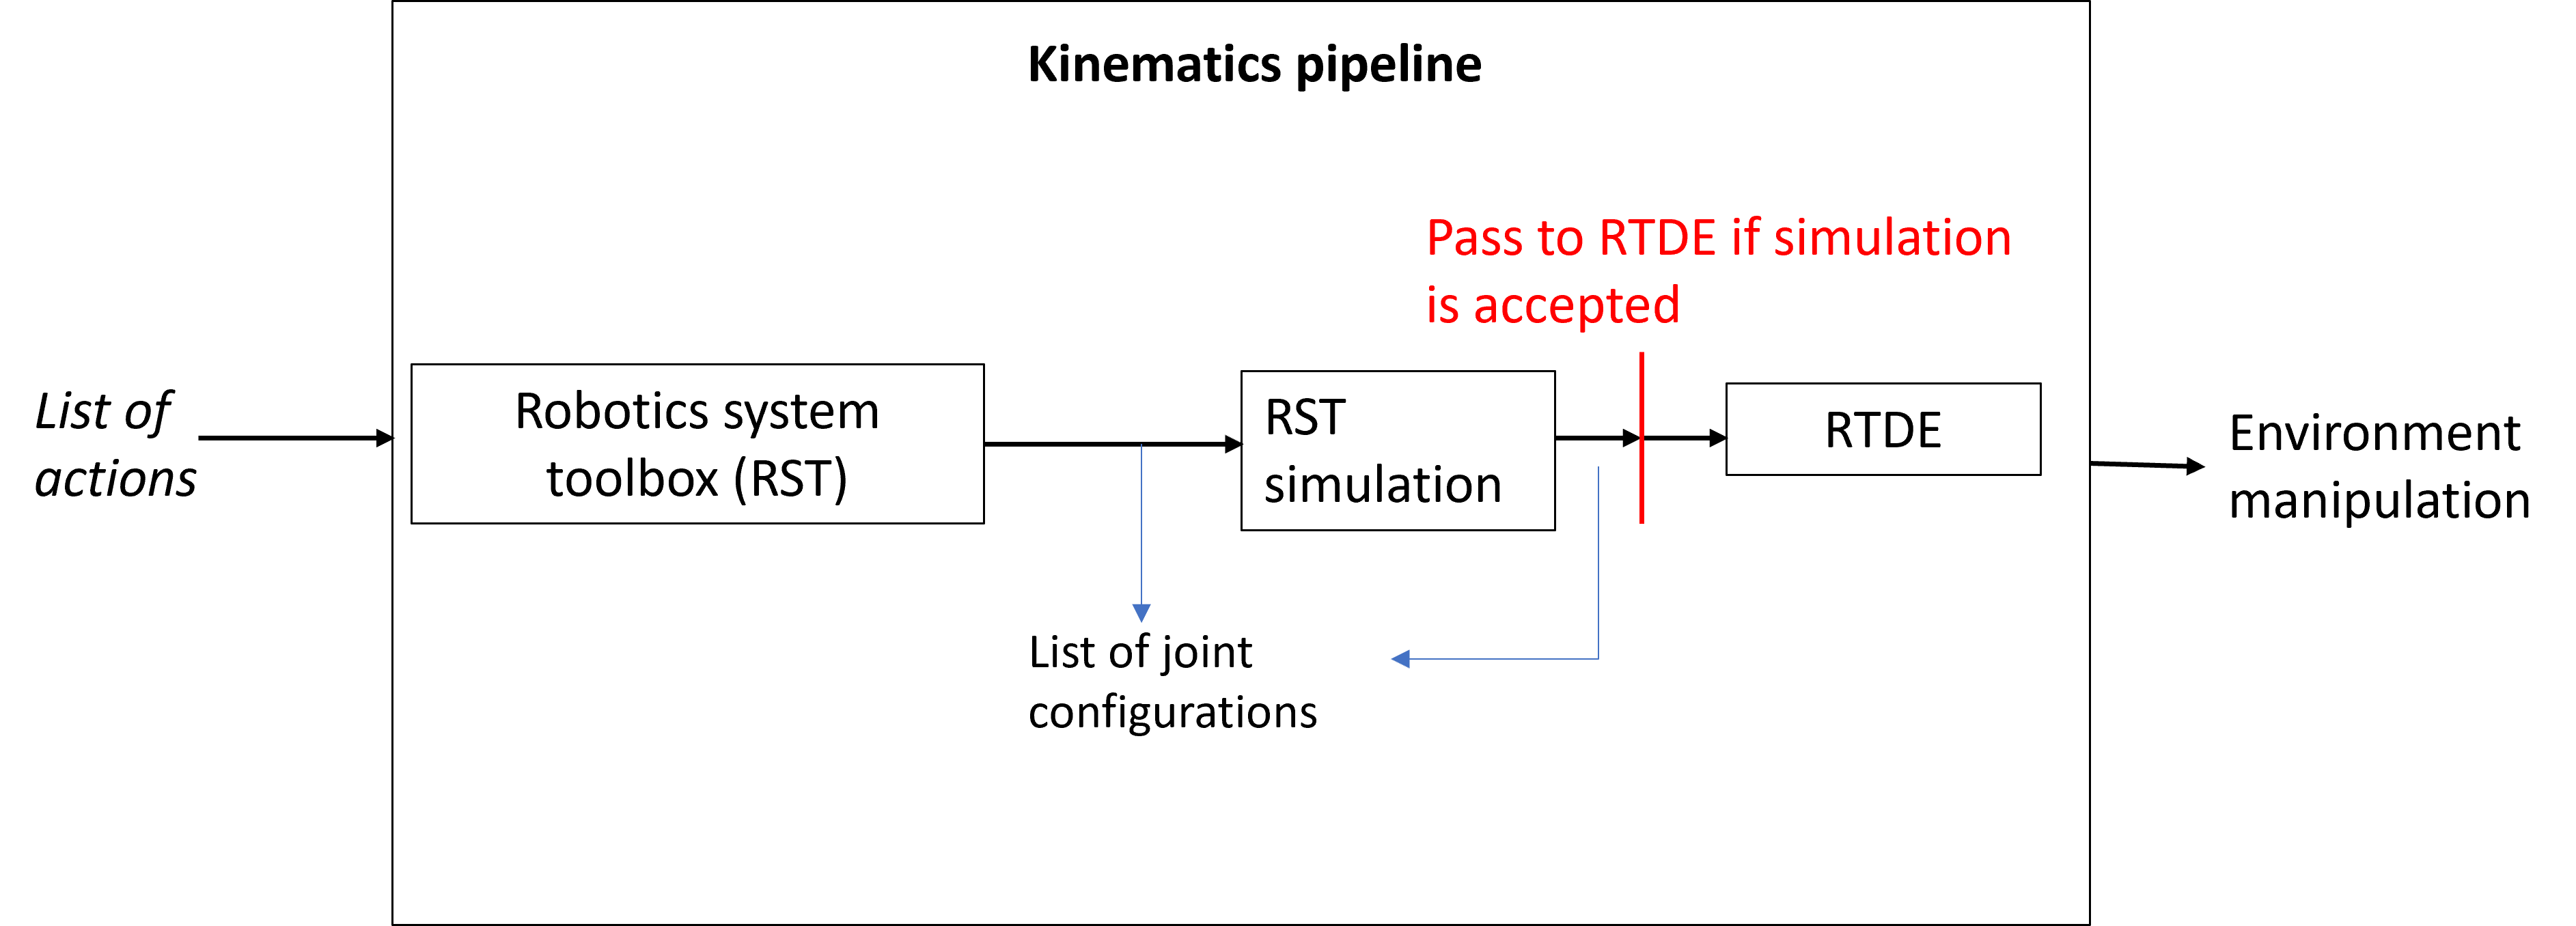
\includegraphics[width=15cm]{img/kinematics_pipeline.png}
    \caption{Figure showing the pipeline for the kinematics part of the system.}
    \label{fig:kin_pipeline}
\end{figure}

For this chapter, the main focus is on the kinematics of the UR5e robot, the software tools used to do the physical operations, and how the pipeline is used to support the system. Furthermore, an explanation is given for how points and frames are created and calculated. The next section introduces the UR5e robot arm and gives a short review of the kinematics of the robot.


\section{UR5e kinematics Introduction}\label{sec:Kinematics_kin_intro}
The UR5e robot arm is the robot manipulator of this system. It is essential to model the kinematics of the robot for the system to be able to control the robot arm. The kinematics of the arm is based on the DH parameters, as the DH parameters transform the coordinate system from the base frame through every joint towards the TCP frame. The DH parameters are shown in table \ref{table:DH_table}. The DH parameters were tabulated from the Universal Robots official website.\footnote{https://www.universal-robots.com/articles/ur/application-installation/dh-parameters-for-calculations-of-kinematics-and-dynamics/}


\begin{table}[ht]
    \centering
    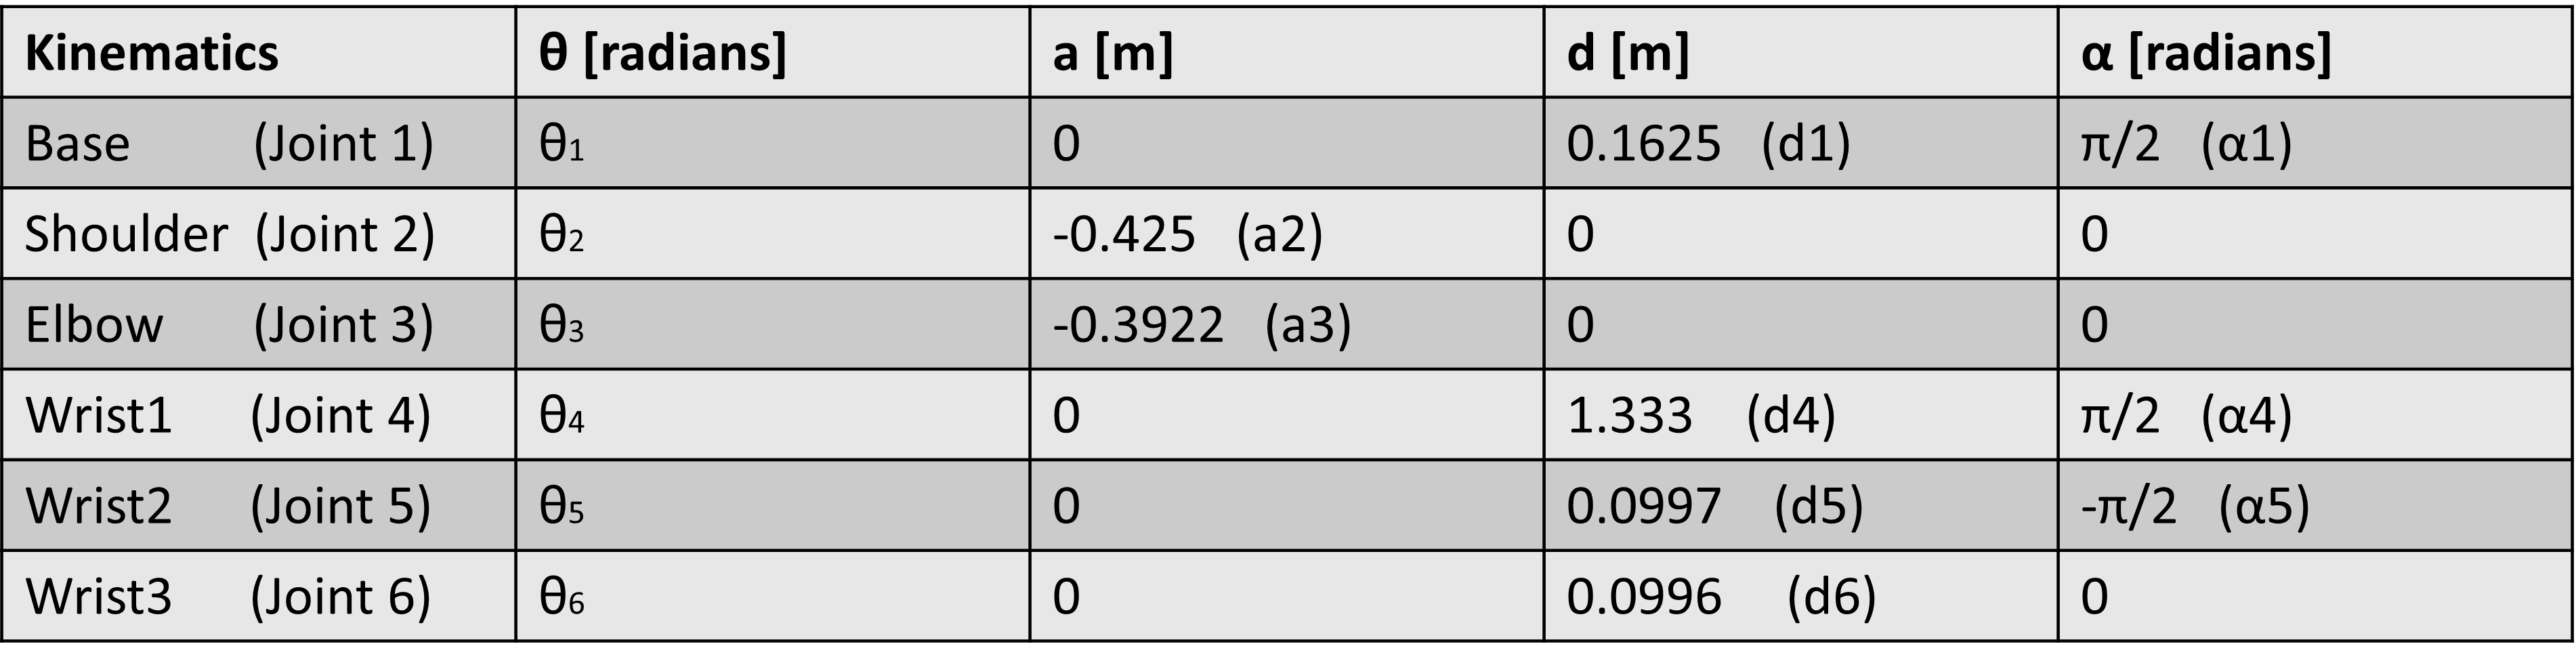
\includegraphics[width=15cm]{img/DH_param_list.png}
    \caption{Table showing the values of the DH parameters for the UR5e robot arm, gotten from Univeral Robots official website.}
    \label{table:DH_table}
\end{table}
Table \ref{table:DH_table} shows the numbers for the DH parameters of the UR5e arm. Figure \ref{fig:DH_UR53} shows a visualization of the given DH parameters. The figure visualizing the DH parameters shows the extension of the UR5e arm links and their natural rotation along the x-axis of each frame. To get a better comparison between the DH parameter visualization and the physical UR5e arm, figure \ref{fig:DH_UR53_theta} is created to show the movable joints of the UR5e arm, placed in the DH parameter visualization. The kinematics of the UR5e robot is now possible to operate with, as the DH parameters are given.
\begin{figure}[ht]
    \centering
    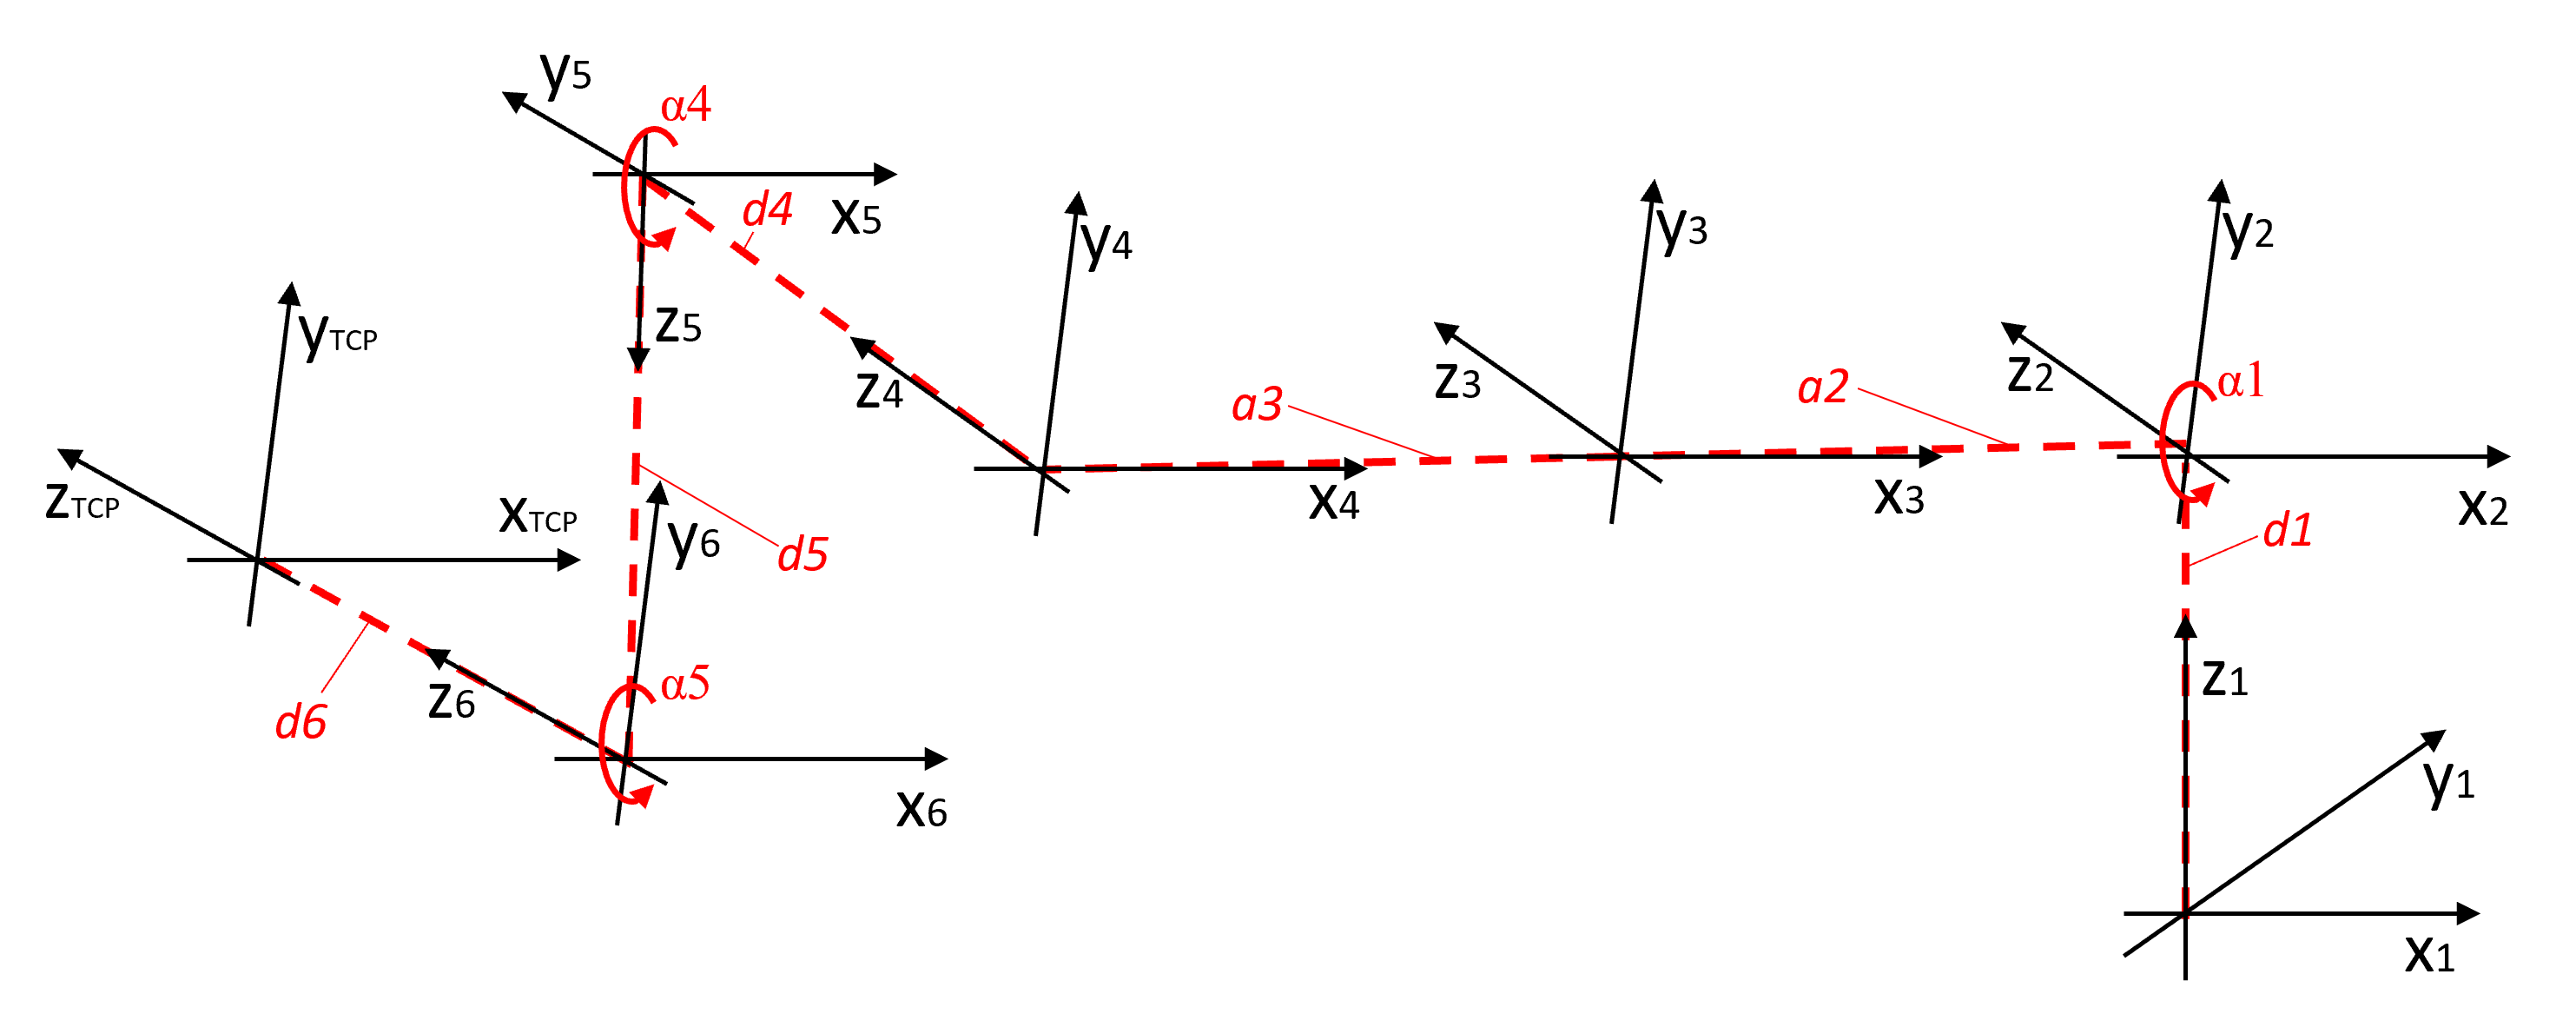
\includegraphics[width=15cm]{img/Wild_DH_parameters.png}
    \caption{Figure illustrating the DH parameters of the robot arm.}
    \label{fig:DH_UR53}
\end{figure}

\begin{figure}[ht]
    \centering
    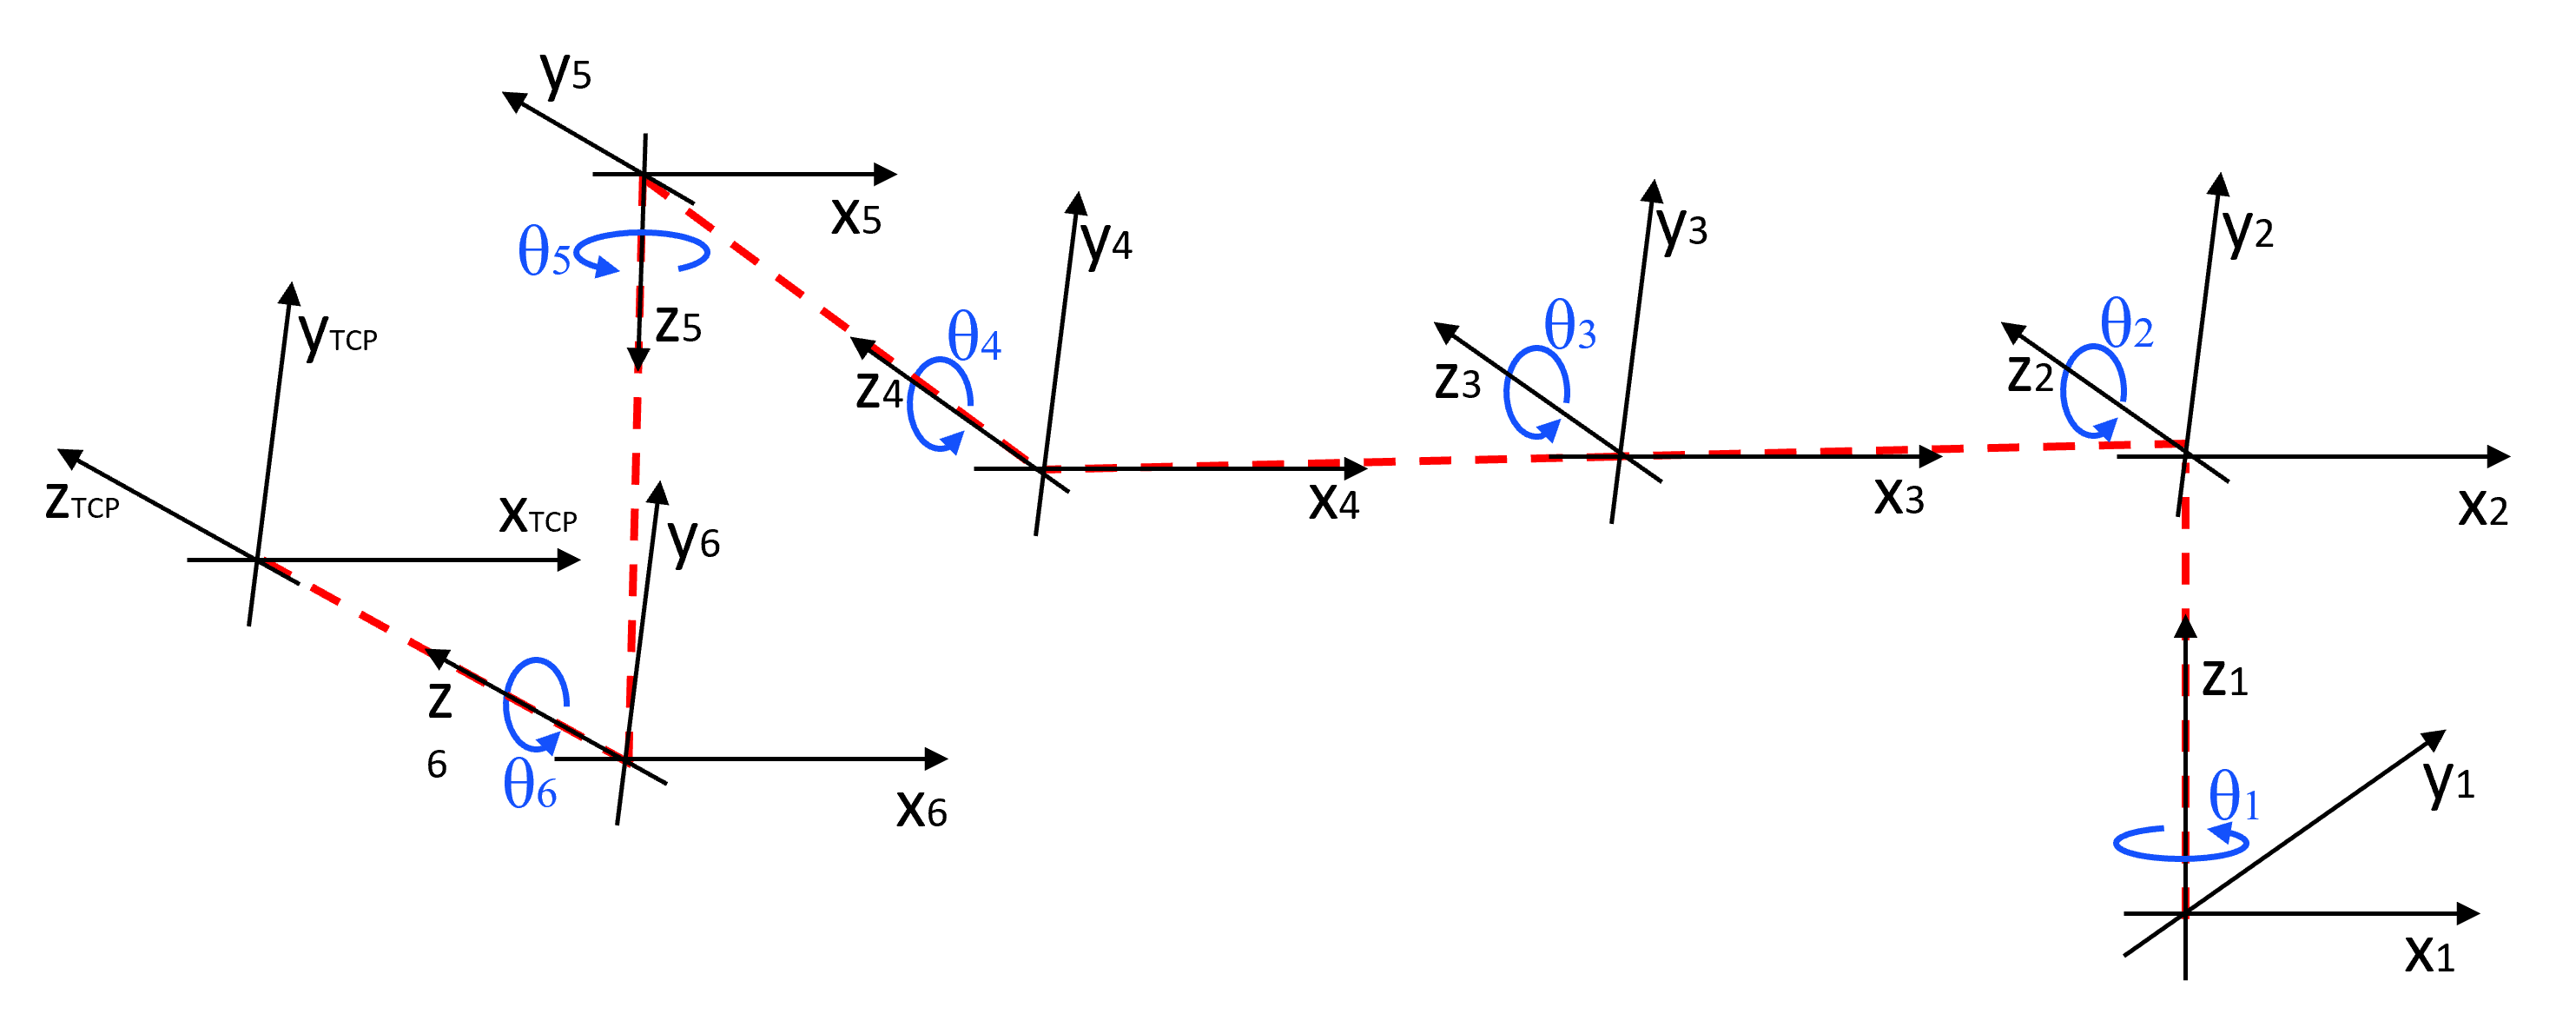
\includegraphics[width=15cm]{img/DH_viz_theta.png}
    \caption{Figure illustrating the movable joints as $\theta$ in the DH parameter visualization.}
    \label{fig:DH_UR53_theta}
\end{figure}

\section{Python robotics system toolbox}\label{sec:Kinematics_pyrst}
For this thesis, the kinematics are handled using the robotics system toolbox (RST) package for Python.
RST is a package used to do kinematics operations on an arbitrary robot, given its DH parameters.
The reason why the kinematics operations are done using this package instead of the UR software itself is that it offers an online robot simulation that can be used to confirm that the robot makes the correct movements. This feature is important for this thesis, as NLP interpretation of natural language instructions might lead to unexpected movements of the robot arm. Therefore, all inverse kinematic operations are handled by the RST package. Figure \ref{fig:RST_kin_pipeline} shows an in-depth explanation of the RST block shown in figure \ref{fig:kin_pipeline} at the start of this chapter.


\begin{figure}[ht]
    \centering
    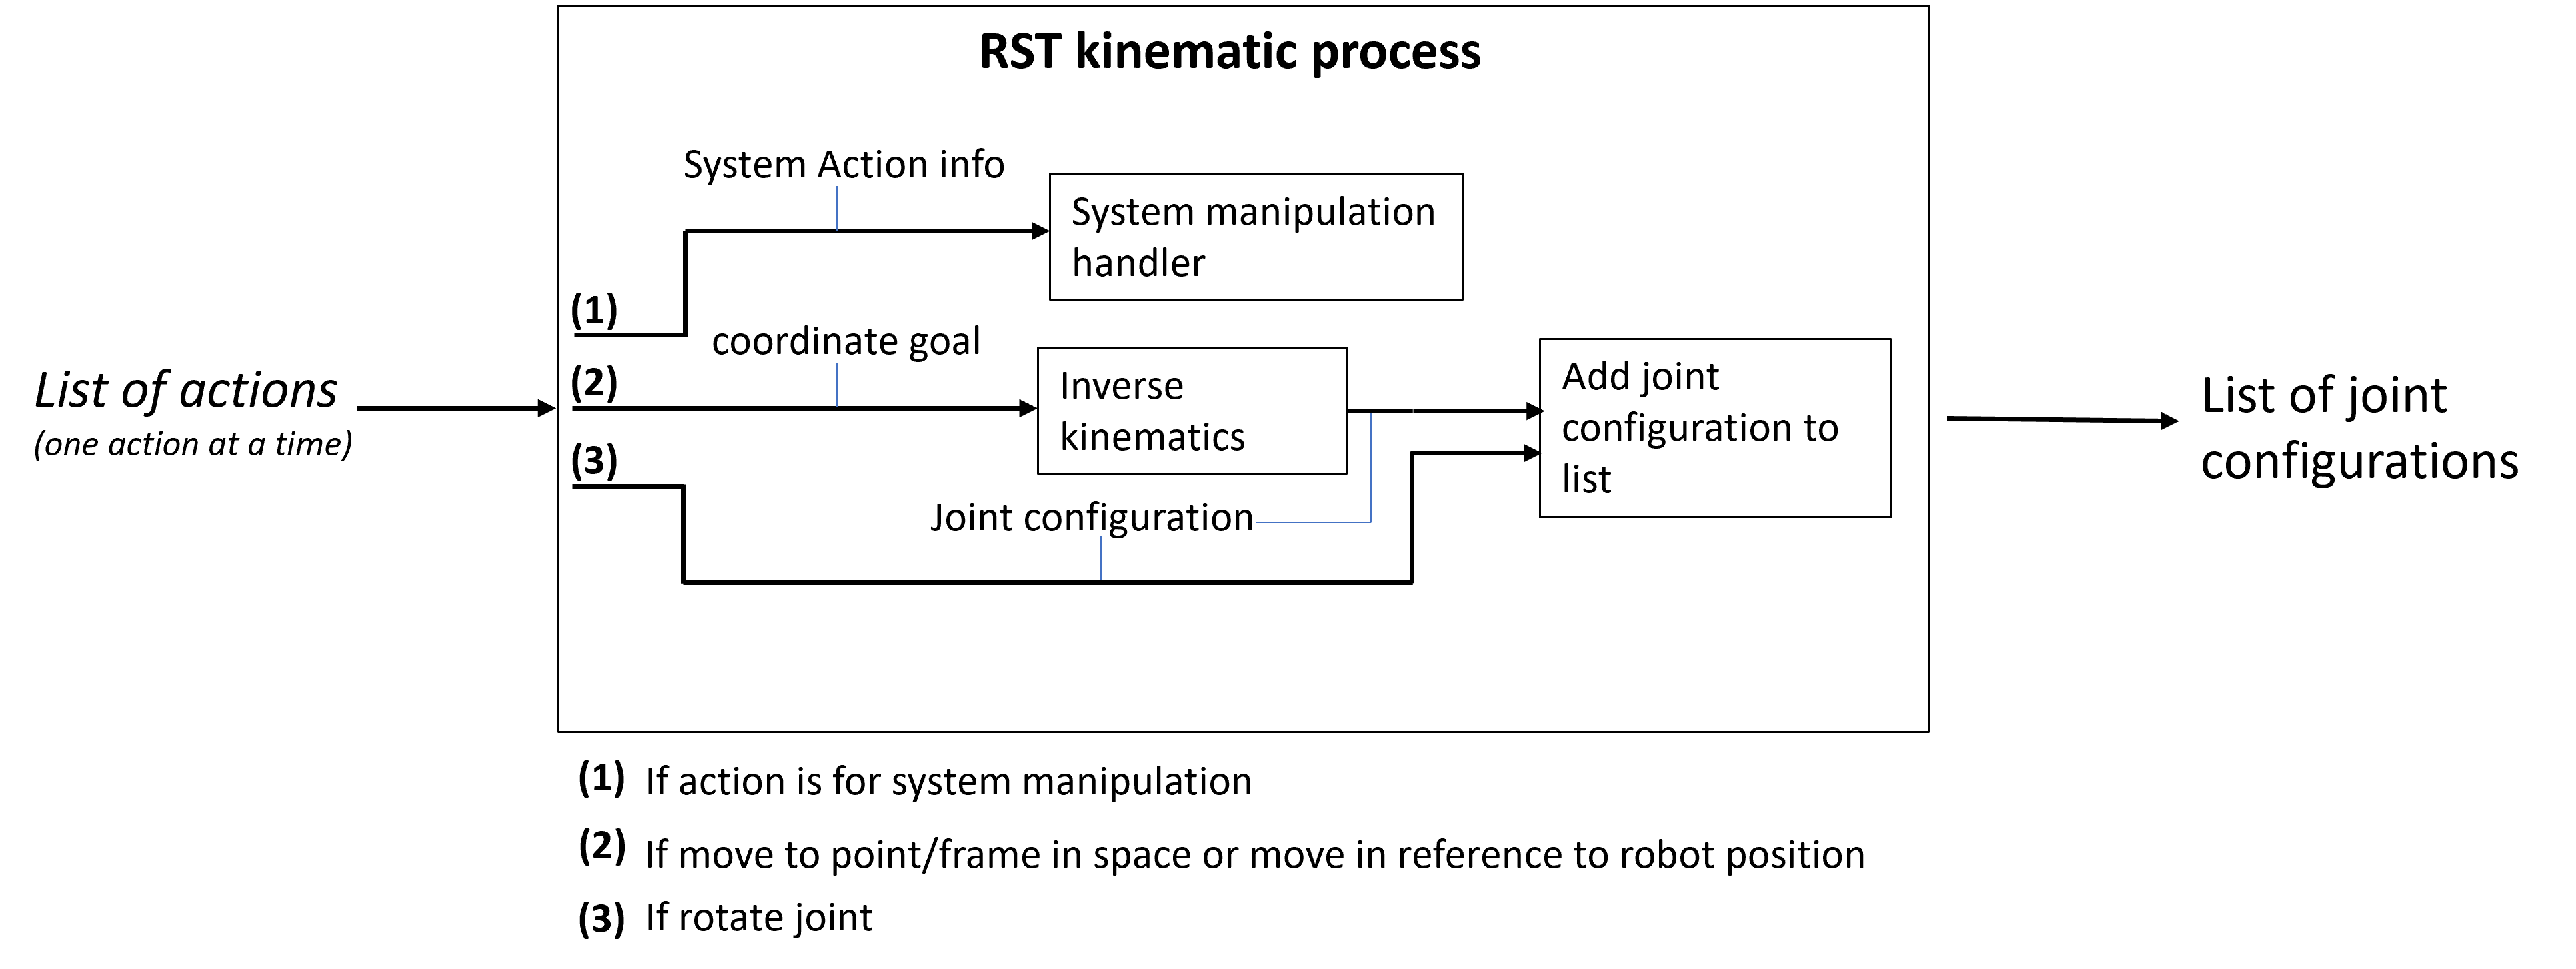
\includegraphics[width=15cm]{img/RST_pipeline.png}
    \caption{Figure illustrating the inner workings of the RST pipeline the numbers indicate requirements for the action object to take the given path.}
    \label{fig:RST_kin_pipeline}
\end{figure}
For figure \ref{fig:RST_kin_pipeline} it should be noted that the actions are passed into the RST kinematics pipeline, one action at a time. The figure shows how each action is processed.
Path \textbf{(1)} shows that an action can be reduced to nothing. This happens if the action in the list of actions does not cause the robot to move but instead is a system manipulation action. For example, \textit{"set position as point 1"} or \textit{"set frame 3 as the current frame"}.
Path \textbf{(2)} is for handling movement to points or frames.
Path \textbf{(3)} is for handling the rotation of joints.
actions moving the robot in reference to itself, such as stated in the instruction \textit{"move 10 cm along the y-axis"} is also in path \textbf{(2)}, as the change in position is viewed by the system as a new point in space that the robot should move to. Though it is viewed as a new point in space, it is not stored in the database.
The kinematics pipeline has access to the same database described in chapter \ref{ch:parser_pipeline}. It, therefore, extracts locations from the database matching the destinations given in the action objects. This is the reason why the list of actions in figure \ref{fig:RST_kin_pipeline} immediately transforms into numerical values in path \textbf{(2)} and \textbf{(3)}. Where the actions become either a coordinate the robot should move to or a joint configuration that indicates a rotation of a single joint.
The inverse kinematics are calculated using a numerical method called LM (Levenberg-Marquadt) with optimization made based on Chan's method.
Though an analytical expression for the inverse kinematics can be created for the UR5e, it is not present in RST. Therefore, RST's inverse kinematics methods are used instead.
The output of the RST process is a list of joint configurations. This is because if both the RST simulator and the UR API use joint configurations to move the robot, then the movements created by the two separate software should be similar. The exact movements might vary based on the velocity profiles of each joint, but this variation has been observed to be small enough, through testing, to be negligible. The exact tests that are referred to are the ones done in chapter \ref{ch:eval}.
A video presentation of the online demonstration of the movement in comparison to the real robot is given at the link below.\footnote{https://www.youtube.com/watch?v=pzW4MFeVL18} The output from RST is passed into the RTDE package, which is used to communicate with the UR5e robot arm. This is discussed in the next section.
\section{RTDE - python package}
A C++ interface for RTDE (Real-Time Data Exchange) wrapped into Python is used to control the UR5e robot arm. It allows a programmer to use UR function commands from Python, given the IP address of the arm. For this specific thesis, two functions are used.
\begin{itemize}
    \item rtde\_receive.getActualQ()
    \item rtde\_control.moveJ(joint\_config)
\end{itemize}
getActualQ() is a function that returns the joint positions of the robot. This function is used to synchronize the system's robot pose with the actual robot pose. This is important for the robot to move relative to its own positions and for the online simulation to start at the correct location.
The function MoveJ(joint\_config) is used to move the joints of the robot to the target joint configuration input, given as joint\_config. As stated before, the reason why RTDE is not used for anything other than the necessary communication is to handle all information in the RST pipeline. Therefore, no more than two functions are used.

\section{Points and frames creation}\label{sec:Kinematics_kin_impl}
The last part of this chapter is about the mathematical operations done to create the points and frames in space and how RST is used to support the operations. The figure from chapter \ref{ch:overview} is given again as figure \ref{fig:kin_point_frame_explanation} to show how the points and frames are linked together. What the figure shows is that points are created in reference to frame coordinate systems in general. Therefore, if a point is created 5 cm along the x-axis of frame 1, then it could also be used as a position 5 cm along the x-axis of any frame.

\begin{figure}[ht]
    \centering
    \begin{subfigure}[b]{0.3\textwidth}
        \centering
        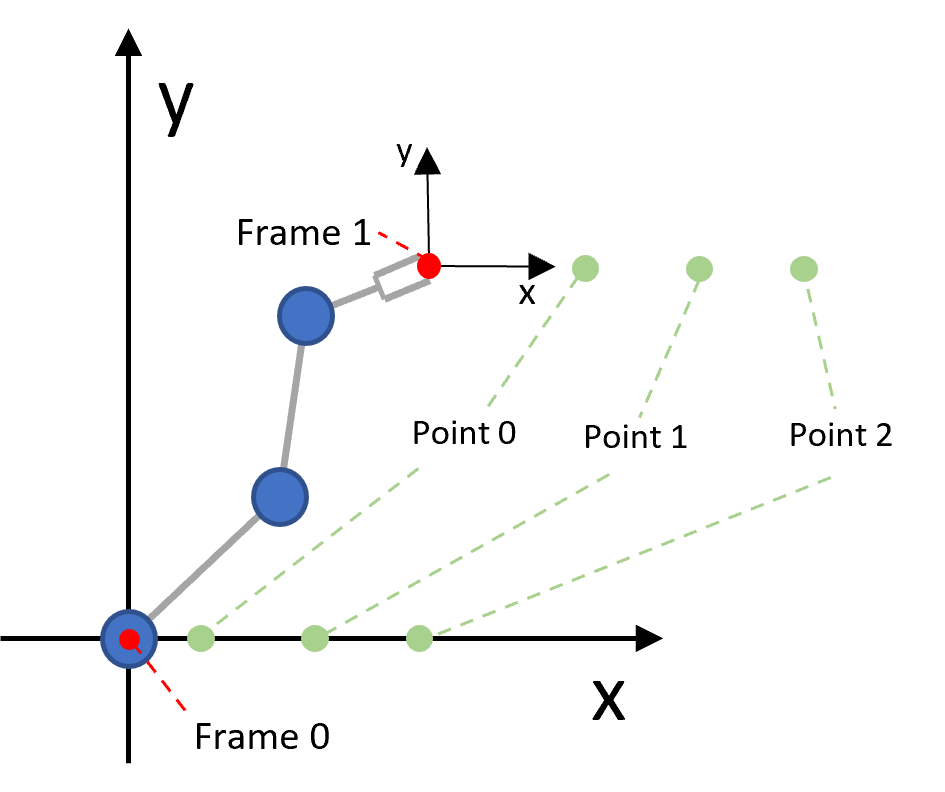
\includegraphics[width=6.5cm]{img/point_frame_explanation1.png}
        \caption{$ $ Visualization of points in frame 1.}
        \label{fig:kin__PF1}
    \end{subfigure}
    \hspace{3cm}
    \begin{subfigure}[b]{0.3\textwidth}
        \centering
        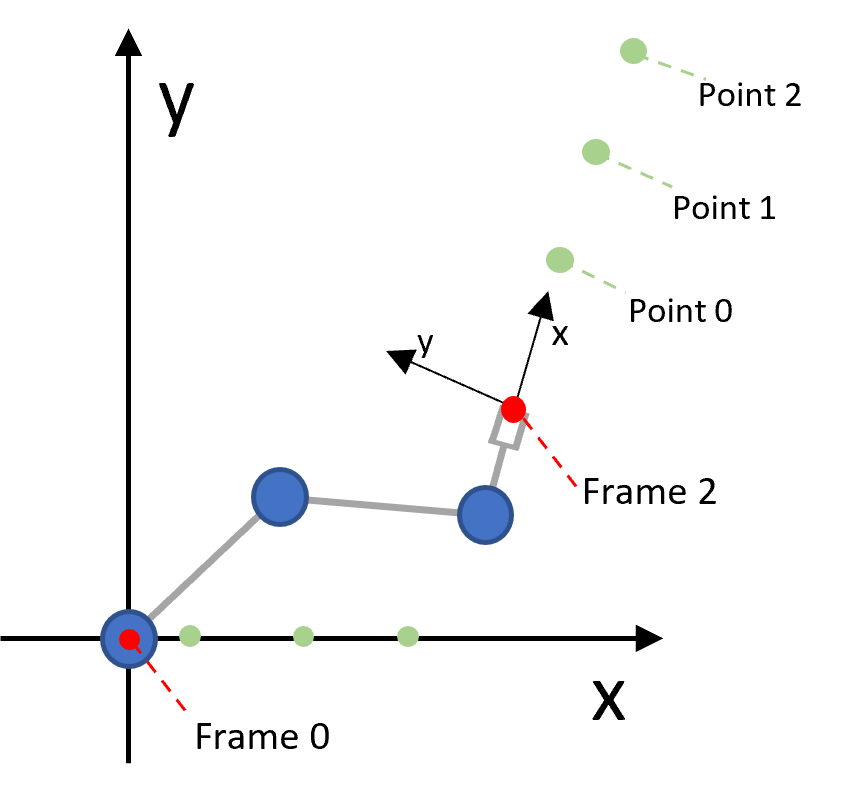
\includegraphics[width=6.5cm]{img/point_frame_explanation2.png}
        \caption{$ $ Visualization of points in frame 2.}
        \label{fig:kim__PF2}
    \end{subfigure}
       \caption{2D visualization of the point frame system created.}
       \label{fig:kin_point_frame_explanation}
\end{figure}

The mathematical operations needed to store the tool center point location in reference to the current frame that the system is working in are therefore given as follows:
$$
\begin{bmatrix}
    ^{A}p_{i + 1}   \\
    1     
\end{bmatrix}
= (_{A}^{O}T_{current})^{-1} \ 
\begin{bmatrix}
    ^{O}p_{tcp}   \\
    1     
\end{bmatrix}
$$
where $^{A}p_{i + 1}$ is a new point in the system, in reference to the current working frame given as a vector. $_{A}^{O}T_{current}$ is the transformation from the base frame (marked as 'O') to the current frame (marked as 'A'), given as a $4\cross 4$ homogeneous transformation. $^{O}p_{tcp}$ is the current location of the tool center point in base frame coordinates. The point $^{O}p_{tcp}$ is calculated by using the RTDE function getActualQ() and then using a forward kinematics function in RST to calculate the tool center point location (disregarding orientation). The point $^{A}p_{i + 1}$ is then written to the database and can be used as a position that the robot can move towards.
To move to point $^{A}p$, it should be transformed back into base frame coordinates. This is done as
$$
\begin{bmatrix}
    ^{O}p_{tcp}   \\
    1     
\end{bmatrix}
=
_{A}^{O}T_{current} \ 
\begin{bmatrix}
    ^{A}p_{i + 1}   \\
    1     
\end{bmatrix}
$$
Afterward, the point location $^{O}p_{tcp}$ is given as input for RST's numeric invers kinematics (along with the robot pose as the initial query). The output from the inverse kinematics function is a joint configuration passed into the RST simulator and then into the RTDE Python function moveJ and executed on the physical robot.
\\
Frames are calculated in a similar way to how TCP location is calculated (using the joint configuration of the robot, then passing it through forward kinematics). The difference is that the orientation is not disregarded and is given along with the translation as a homogeneous transformation.
